\chapter{常用物理常数}
\href{https://en.wikipedia.org/wiki/List_of_physical_constants}{物理常数表}
\section{SI单位制}
\paragraph{基本单位}
\begin{center}
	\captionof{table}{SI基本单位}
	\begin{tabular}{ccc}
		\toprule
		物理量&单位&定义\\
		\midrule
		时间&s&$^\ast$\\
		长度&m&光速$c$\\%和s\\
		质量&kg&Planck常数$h$\\%和m, s\\
		电流&A&元电荷$e$\\%和s\\
		热力学温度&K&Boltzmann常数$\kB$\\%和kg, m, s\\
		物质的量&mol&Avogadro常数$\NA$\\
		发光强度&cd&$^{\ast\ast}$\\
		\bottomrule
	\end{tabular}
\end{center}
$^\ast\enspace$基态$\nucli{133}{Cs}$超精细能级跃迁频率$\nu=\SI{9192631770}{Hz}$\\
\noindent
$^{\ast\ast}\enspace f=\SI{540E12}{Hz}$的单色辐射源辐射强度为$\frac1{683}\,\si{W/sr}$
\paragraph{词头}
\begin{center}
	\captionof{table}{SI词头}
	\begin{tabular}{ccc|ccc}
		\toprule
		名称&符号&系数&名称&符号&系数\\
		\midrule
		十&da&$10^1$&分&d&$10^{-1}$\\
		百&h&$10^2$&厘&c&$10^{-2}$\\
		千&k&$10^3$&毫&m&$10^{-3}$\\
		兆&M&$10^6$&微&\si{\ \micro\ }&$10^{-6}$\\
		吉&G&$10^9$&纳&n&$10^{-9}$\\
		太&T&$10^{12}$&皮&p&$10^{-12}$\\
		拍&P&$10^{15}$&飞&f&$10^{-15}$\\
		艾&E&$10^{18}$&阿&a&$10^{-18}$\\
		泽&Z&$10^{21}$&仄&z&$10^{-21}$\\
		尧&Y&$10^{24}$&幺&y&$10^{-24}$\\
		\bottomrule
	\end{tabular}
\end{center}
\paragraph{导出单位}
\begin{center}
	\captionof{table}{SI基本单位}
	\begin{tabular}{ccc}
		\toprule
		物理量&单位&基本单位表达\\
		\midrule
		角&rad&\\
		立体角&sr&\\
		频率&Hz&\si{s^{-1}}\\
		力&N&\si{kg.m/s^{-2}}\\
		压强&Pa&\si{kg/m.s^{-2}}\\
		能量、功&J&\si{kg.m^2/s^{-2}}\\
		功率、辐射通量&W&\si{kg.m^2/s^{-3}}\\
		电荷&C&\si{A.s}\\
		电压&V&\si{kg.m^2/A.s^3}\\
		电容&F&\si{A^2.s^4/kg.m^2}\\
		电阻&$\Omega$&\si{kg.m^2/A^2.s^3}\\
		电导&S&\si{A^2.s^3/kg.m^2}\\
		电感&H&\si{kg.m^2/A^2.s^2}\\
		磁通量&Wb&\si{kg.m^2/A.s^2}\\
		磁感应强度&T&\si{kg/A.s^2}\\
		摄氏度&$\si{\degreeCelsius}$&K\\
		光通量&lm&cd\\
		照度&lx&\si{cd/m^2}\\
		放射性活度&Bq&\si{s^{-1}}\\
		\bottomrule
	\end{tabular}
\end{center}
\section{SI单位制定义的准确值}
\begin{compactitem}
	\item 真空中光速
		\begin{align}
			c:=\SI{299792458}{m/s}.
		\end{align}
	\item Planck常数
		\begin{align}
			h:=\SI{6.62607015E-34}{J.s}
		\end{align}
		约化Planck常数
		\begin{align}
			\hbar:=\frac{h}{2\pi}=\SI{1.05457182E-34}{J.s}.
		\end{align}
	\item 电荷单位(elementary charge)
		\begin{align}
			e:=\SI{1.602176634E-19}{C}.
		\end{align}
		数值上,单位电子伏eV等于电荷单位的J.
	\item Boltzmann常数
		\begin{align}
			\kB:=\SI{1.380649E-23}{J/K}.
		\end{align}
	\item Avogadro常数
		\begin{align}
			\NA:=\SI{6.02214076E23}{mol^{-1}}.
		\end{align}
\end{compactitem}
\paragraph{由定义推导出的准确物理常数}~
\begin{compactitem}
	\item 理想气体常数
		\begin{align}
			R:=\kB\NA=\SI{8.314462618}{J/K.mol}
		\end{align} % 15324
	\item Faraday常数
		\begin{align}
			F:=\NA e=\SI{9.648533212E4}{C/mol}
		\end{align} % 33100184
	\item Stefan-Boltzmann常数
		\begin{align}
			\sigma:=\frac{2\pi^5\kB^4}{15h^3c^2}=\SI{5.670374419E-8}{W/m^2.K^4}
		\end{align} % 184429453971
	\item Wein位移定律常数
		\begin{align}
			\lambda\maxi T=\frac{hc}{\xi\kB}=\SI{2.897771955}{mm.K}
		\end{align} % 185172661
		$\xi=\num{4.965114232}\ldots$是方程$\xi=5(1-\e{-\xi})$的解。
	\item 第一辐射常数(first radiation constant)
		\begin{equation}
			c_1=2\pi hc^2=\SI{3.741771852E-16}{W.m^2}.
		\end{equation} % 192758011367103884
	\item 第二辐射常数(second radiation constant)
		\begin{equation}
			c_2=\frac{hc}\kB=\SI{1.4387768775E-2}{m.K}.
		\end{equation} % 03933802146671602
\end{compactitem}
\section{常用的物理常数}
\sisetup{separate-uncertainty = false}
\begin{itemize}
	\item 万有引力常数(gravitational constant)
		\begin{align}
			G=\SI{6.67430(15)e-11}{m^3/kg.s^2}
		\end{align}
	
	\item 真空介电常数(permittivity of free space)
		\begin{align}
			\varepsilon_0=\SI{8.8541878128(13)E-12}{F/m};
		\end{align}
		真空磁导率(permeability of free space)
		\begin{align}
			\mu_0=\SI{1.25663706212(19)E-6}{H/m};
		\end{align}
		一个非常接近的值是旧SI单位制下用来定义A的$\mu_0$
		\[
			\mu_0:=4\pi\times 10^{-7}\,\si{H/m},
		\]
		自由空间阻抗(impedance of free space)
		\begin{equation}
			Z_0:=\sqrt{\frac{\mu_0}{\varepsilon_0}}=\SI{376.730313412(59)}{\ohm}
		\end{equation}
		由于$c=1/\sqrt{\varepsilon_0\mu_0}$;有近似值$Z_0=\mu_0c\simeq 120\pi\,\si{\ohm}.$
	
	\item 精细结构常数(fine-structure constant)
		\begin{align}
			\alpha:={}&\frac{e^2}{4\pi\varepsilon_0}\frac1{\hbar c}=\num{7.2973525693(11)E-3};\\
			\alpha^{-1}={}&\num{137.035999084(21)}.
		\end{align}
	
	\item 原子质量单位
		\begin{align}
			\SI{1}{u}=\frac{M(\nucli{12}{C})}{12}=\SI{1.66053906660(50)E-27}{kg}.
		\end{align}
		一个非常接近的值是旧SI单位制下Avogadro常数的定义:
		\[
			\SI{1}{u}=\frac1{\NA}\,\si{g}.
		\]
	
	\item 电子、质子、中子质量
		\begin{align}
			m_\elc&=\SI{9.1093837015(28)E-31}{kg}\\
			&=\SI{5.48579909065(16)E-4}{u}\\
			&=\SI{0.51099895000(15)}{MeV}/c^2.\\
			m_\pton&=\SI{1.67262192369(51)E-27}{kg}\\
			&=\SI{1.00866491588(49)}{u}\\
			&=\SI{938.27208816(29)}{MeV}/c^2;\\
			m_\nton&=\SI{1.67492749804(95)E-27}{kg}\\
			&=\SI{1.007276466621(53)}{u}\\
			&=\SI{939.56542052(54)}{MeV}/c^2.
		\end{align}
		质子电子质量比
		\begin{align}
			\frac{m_\pton}{m_\elc}=\num{1836.15267343(11)}.
		\end{align}
		电子荷质比
		\begin{align}
			\frac e{m_\elc}=\SI{1.75882E11}{C/kg}.
		\end{align}
	
	\item 电子Compton波长和约化Compton波长
		\begin{align}
			\lambda_\elc&=\frac h{m_\elc c}=\SI{2.42631023867(73)}{pm};\\
			\lambdabar_\elc&=\frac{\lambda_\elc}{2\pi}=\SI{3.861 592 6796(12)E-13}{m}.
		\end{align}
	
	\item 经典电子半径
		\begin{align}
			r_\elc:=\frac{e^2}{4\pi\varepsilon_0}\frac1{m_\elc c^2}=\alpha\lambdabar_\elc=\SI{2.8179403262(13)}{fm}
		\end{align}
		Thomson散射截面
		\begin{align}
			\sigma_\elc:=\frac{8\pi}3r_\elc^2=\SI{6.6524587321(60)E-29}{m^2}.
		\end{align}
	
	
	
	\item Bohr半径
		\begin{align}
			a_0:=\frac{4\pi\varepsilon_0}{e^2}\frac{\hbar^2}{m_\elc}=\frac{r_\elc}{\alpha^2}=\SI{5.29177210903(80)E-11}{m}.
		\end{align}
	\item Rydberg常量
		\begin{align}
			R_\infty:=\frac{\alpha^2}{2\lambda_\elc}=\SI{10973731.568160(21)}{m^{-1}}
		\end{align}
		Rydberg单位能量
		\begin{align}
			\SI{1}{Ry}:=\frac{e^2}{4\pi\varepsilon_0\cdot 2a_0}=\SI{2.1798723611035(42)e-18}{J}
		\end{align}
	
	\item Bohr磁子
		\begin{align}
			\muB:=\frac{e\hbar}{2m_\elc}=\SI{9.2740100783(28)E-24}{J/T}
		\end{align}
\end{itemize}
\paragraph{常用常数组合}
\begin{align}
	hc&=\SI{1.986445857E-25}{J.m}\\ % 14892870
	&=\SI{1.239841984E-6}{eV.m}\\  % 332002622377527446
	\hbar c&=\SI{3.161526773E-26}{J.m}\\ % 496689987889773799
	&=\SI{1.97326980459E-7}{eV.m}\\ % 3024658908971331
	\frac{e^2}{4\pi\varepsilon_0}&=\SI{2.307077552E-28}{J.m}\\ % 341736287791637868
	&=\SI{1.4399645478E-9}{eV.m} % 42567205852558868
\end{align}
$\SI{1}{eV}$对应频率
\begin{equation}
	\nu_0=\frac eh=\SI{2.417989242E14}{Hz}
\end{equation} % 084918162238291425
$\SI{1}{eV}$对应波数
\begin{equation}
	k_0=\frac e{hc}=\SI{8.065543937E5}{m^{-1}}
\end{equation} % 349211641069007231

\chapter{元素周期表}

\begin{figure}[h]
	\centering
	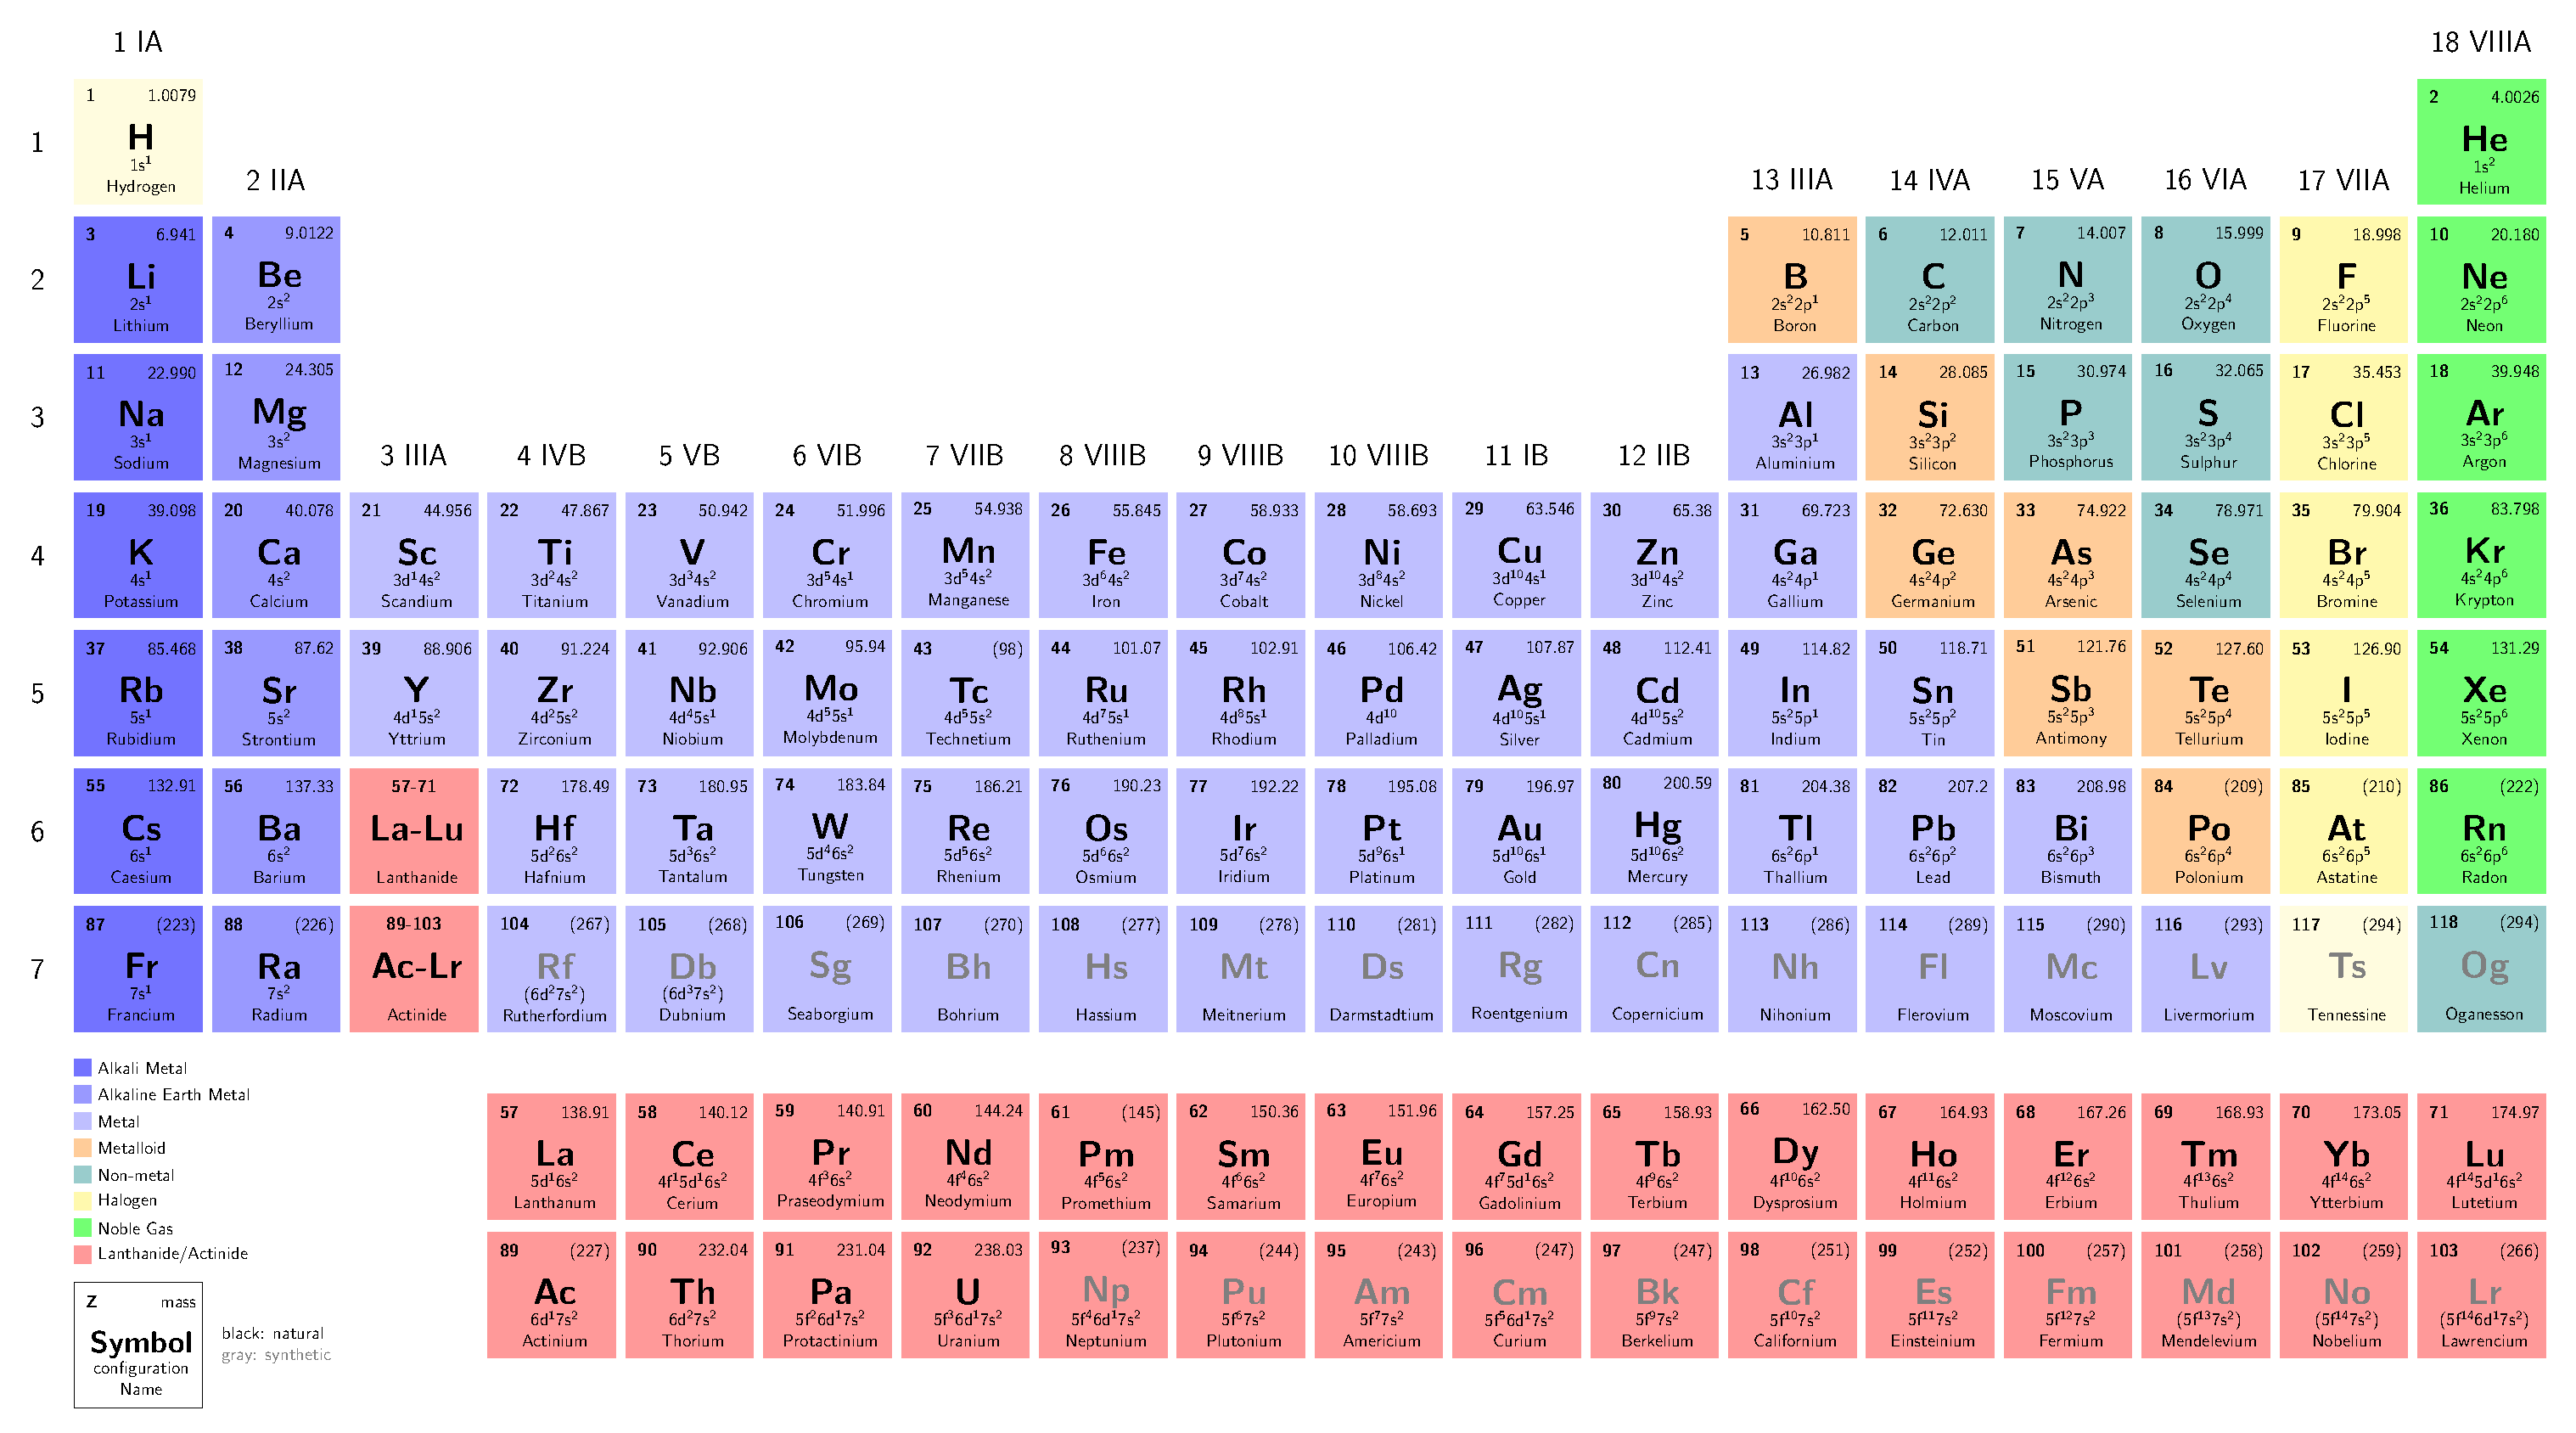
\includegraphics[width=\linewidth]{figures/tikz/periodic_table.pdf}
	\caption{元素周期表}
	\label{fig:periodic_table}
\end{figure}

ref: \href{https://texample.net/tikz/examples/periodic-table-of-chemical-elements}{Periodic Table of Chemical Elements}.

All Credit to Ivan Griffin.

\chapter{放射系}

\begin{figure}[h]
	\centering
	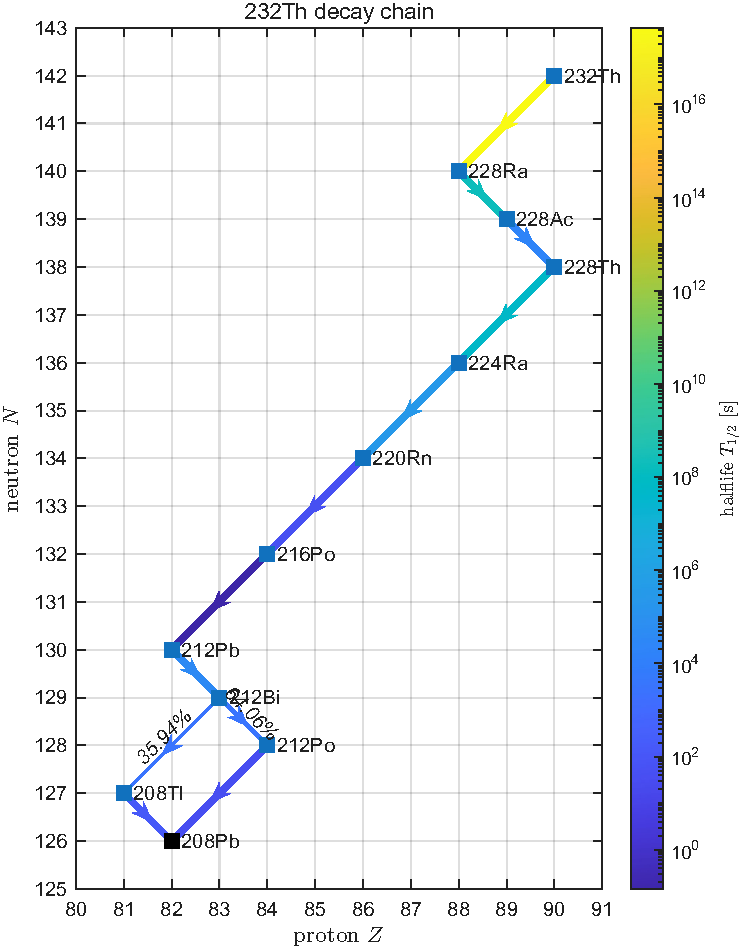
\includegraphics[page=1]{figures/decay_system.pdf}
	\caption{钍系$\nucli{232}{Th}$衰变图}
	\label{fig:decay_system 232Th}
\end{figure}

\begin{figure}[hp]
	\centering
	\includegraphics[page=2]{figures/decay_system.pdf}
	\caption{铀系$\nucli{238}{U}$衰变图}
	\label{fig:decay_system 238U}
\end{figure}

\begin{figure}[hp]
	\centering
	\includegraphics[page=3]{figures/decay_system.pdf}
	\caption{锕铀系$\nucli{235}{U}$衰变图}
	\label{fig:decay_system 235U}
\end{figure}



% \printindex


